\graphicspath{{introduction/fig/}}

\chapter{Introduction}
\label{chap:introduction}

\begin{quote}
    "We don't tell [computers] what to do, we give them examples... The problem is, sometimes we don't understand how it figured it out."\\ % <--- FORCED NEW LINE HERE
    \vspace{0.5em} % Adds a slightly larger vertical space after the quote text
    \hfill -- Jeff Dean, Head of Google AI \cite{Dean2017BlackBox}
\end{quote}

The prevalence of neural networks (NNs) has established them as a foundational technology in modern artificial intelligence. However, as their use has expanded, so too has attention to their inherent mechanistic limitations. Two major drawbacks of NNs are their lack of explainability—the “black-box” effect—and the substantial computational cost of training. With platforms like Hugging Face and GitHub hosting over one million pre-trained models \cite{huggingface2024review}, interest in addressing these limitations has intensified. Motivated by this vast availability of models, a novel research direction—weight space learning—has emerged as a promising approach to better understand these limitations.

Formally, the weight space of a neural network refers to the set of all possible configurations of its parameters \( W \in \mathbb{R}^n \), where \( n \) is the total number of trainable weights. Each point in this space represents a unique model with a distinct mapping from inputs to outputs. Weight space learning thus concerns learning representations or distributions over this space, capturing how variations in \( W \) relate to model behaviour and how variations in model training influence \( W \). The field generally considers two types of tasks: discriminative and generative.

In discriminative applications, models use the weights of pre-trained networks—often collected into a model zoo \cite{schurholt2022modelzoosdatasetdiverse}—as input to predict meta-information about the original models \cite{unterthiner2021predictingneuralnetworkaccuracy}. The quality of a weight space representation is typically evaluated by the performance of a simple multi-layer perceptron (MLP) in predicting such meta-information, conditioned only on the model's weight embedding.

Common meta-information metrics include the model's final performance and its generalisation gap (the difference between training and validation loss). \cite{salama2024datasetsizerecoverylora} demonstrated that weight embeddings can encode key training characteristics, such as recovering the size of the dataset used for training. These discriminative tasks serve both to validate the quality of the derived weight representations and to provide practical predictive value.

In generative applications, researchers aim to model the underlying distribution of neural network weights \( W \), conditioned on additional information or reference models, \( P(W \mid \dots) \). Sampling from this distribution enables the generation of entirely new model weights.

\cite{schurholt2022hyperrepresentationsgenerativemodelssampling} used an autoencoder with a bottleneck layer to generate hyper-representations of multiple model zoos. Building on this idea, \cite{pmlr-v235-schurholt24a} introduced the Sequential Autoencoder for Neural Embeddings (SANE), which improved scalability and enabled work on much larger models.

To model \( P(W \mid \mathcal{D}) \), \cite{bedionita2025instructionguidedautoregressiveneuralnetwork} employed a Vector Quantised Variational Autoencoder (VQ-VAE), which incorporates dataset information when learning latent weight representations. Similarly, \cite{meynent2025structureenoughleveragingbehavior} modelled \( P(W \mid R) \) by incorporating behavioural differences between reconstructed and original models into the embedding learning process.

While existing weight space learning methods have made significant progress, they typically address isolated aspects of the learning process. Current approaches model either \( P(W \mid \mathcal{D}) \) or \( P(W \mid R) \), but rarely both simultaneously. This is a key limitation: in practice, a model's weights are influenced by both the data it was trained on and the results it achieved. Understanding the joint relationship \( P(W \mid \mathcal{D}, R) \) is essential for explaining model behaviour and for generating models with desired characteristics.

Contrastive learning has emerged as a powerful paradigm for learning unified representations across modalities, as demonstrated by models such as CLIP \cite{radford2021learningtransferablevisualmodels}, which bridge vision and language. A contrastive objective pulls related samples closer in representation space while pushing unrelated samples apart, forming a meaningful joint embedding space for heterogeneous data types. This property makes contrastive learning particularly suitable for modelling the complex distribution \( P(W \mid \mathcal{D}, R) \) --- encompassing visual datasets, high-dimensional weight tensors, and performance metrics --- without requiring a shared native representation.

\begin{figure}[!t]
    \centering
    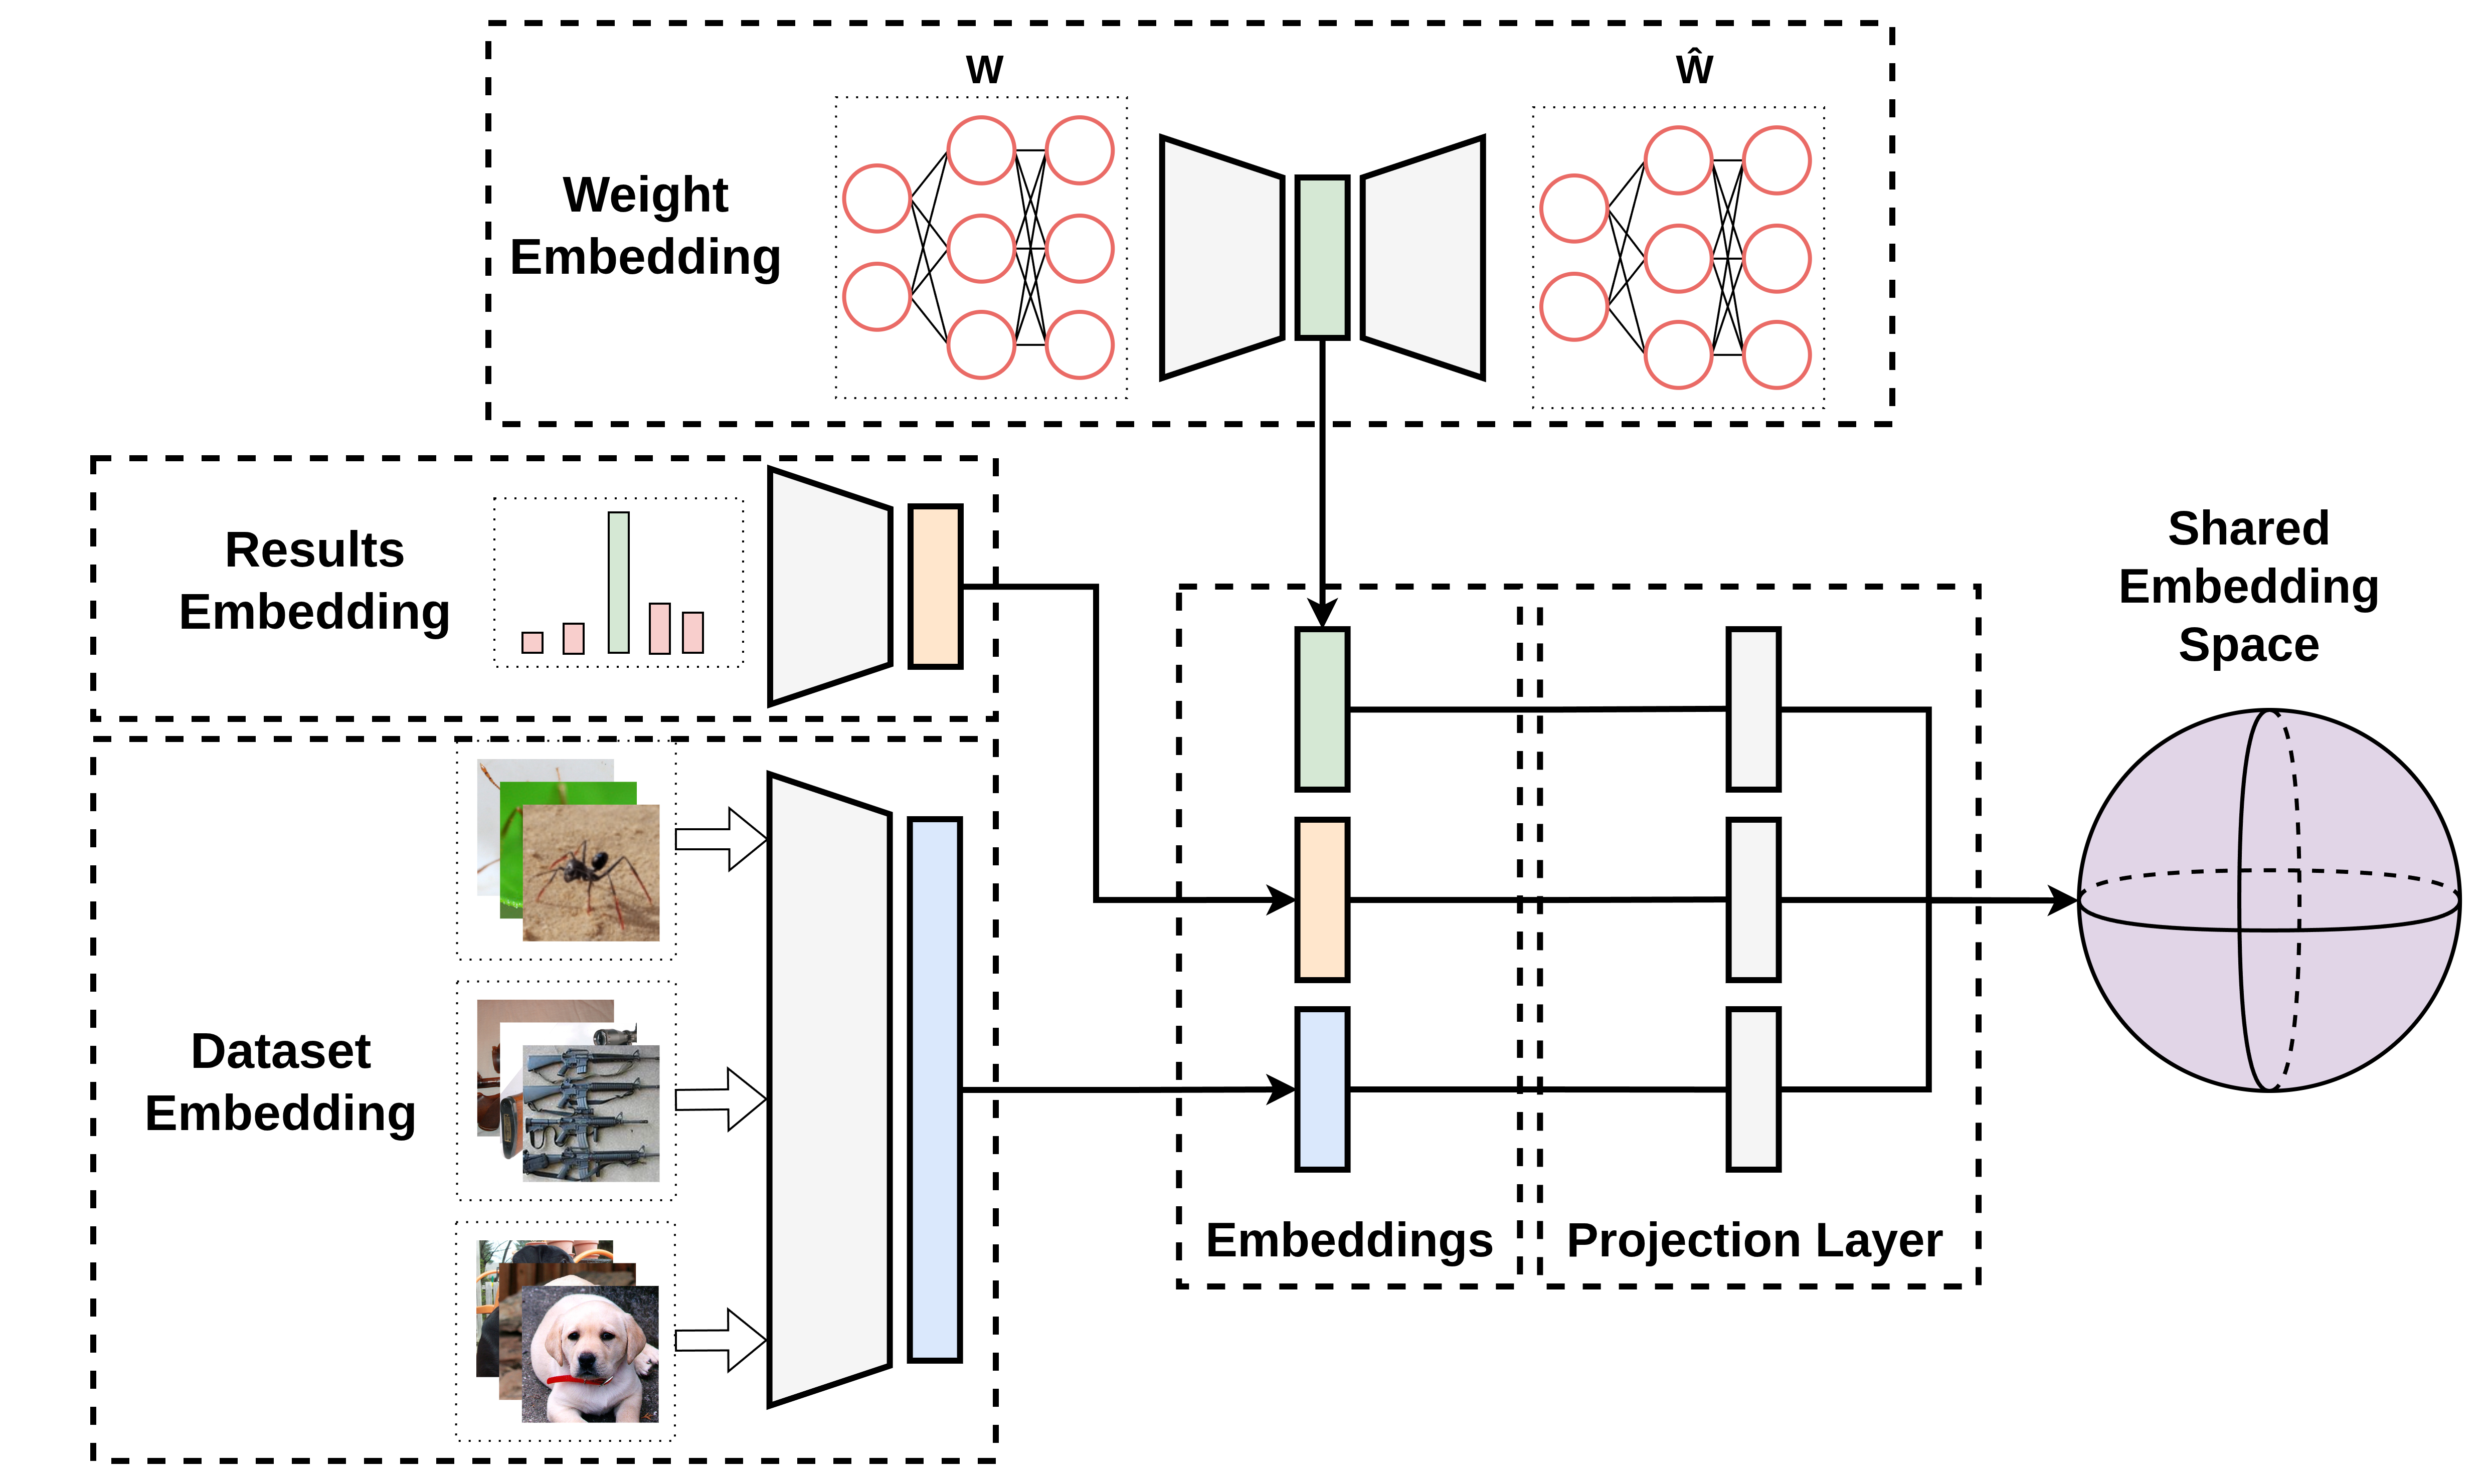
\includegraphics[width=0.75\linewidth]{pipeline.png}
    \caption[A figure illustrating the process of embedding a dataset, model weigths and results into a shared embedding space ]{AA figure illustrating the process of embedding a dataset, model weights and results in a shared embedding space. }
    \label{fig:pipeline}
\end{figure}

In this report, we develop a contrastive learning framework to create a unified embedding space that jointly represents neural network weights \( W \), the datasets they were trained on \( \mathcal{D} \), and their resulting performance characteristics \( R \). Specifically, we construct two separate encoders—one for dataset embeddings using pre-trained CLIP features, and another for weight embeddings using an autoencoder architecture—alongside a binned result embedding table. These encoders are trained using the contrastive objective NT-Xent \cite{agren2022ntxentlossupperbound}, which encourages related triplets \( (\mathcal{D}, W, R) \) to be close in the shared latent space. Figure \ref{fig:pipeline} depicts a high-level view of the full embedding pipeline.



Our central hypothesis is that this unified representation space will enable two key capabilities:

\textbf{Interpretability and Analysis:} Examining geometric relationships within the shared embedding space can reveal how dataset characteristics shape learned weights and model behaviour. By establishing a meaningful relationship between the triplet \( (\mathcal{D}, W, R) \), one can systematically perturb any of the three components while keeping the others fixed, and observe how such changes affect the reconstructed---and thus the real---weight space. This capability enables a structured and extensive exploration of how dataset properties and training outcomes influence learned representations.

\textbf{Conditional Model Sampling:} The learned distribution enables sampling of model weights conditioned on both dataset properties and target performance metrics--approximating \( P(W \mid \mathcal{D}, R) \). Such a capability supports zero-shot model generation, where high-performing networks can be synthesised directly from their latent representations, bypassing the need for gradient-based optimisation. By leveraging the structure of the learned weight manifold, this approach has the potential to significantly reduce training costs while enabling the targeted creation of models optimised for specific datasets or performance objectives.

% TODO {introduction}

The results found from the report, and how it's limited 

The remainder of this report is structured as follows.:
    In Section 1 we will discuss x, next y, concluded by z in attempt to showcase that this report is the best
% TODO {introduction}


% \section{Section heading}

% This is some section with two table in it: Table~\ref{tbl:exemplars} and Table~\ref{tbl:abx_speaker}.

% \begin{table}[!h]
%     \mytable
%     \caption{Performance of the unconstrained segmental Bayesian model on TIDigits1 over iterations in which the reference set is refined.}
%     \begin{tabularx}{\linewidth}{@{}lCCCCC@{}}
%         \toprule
%         Metric     & 1 & 2 & 3 & 4 & 5 \\
%         \midrule
%         WER (\%)                        & $35.4$ & $23.5$ & $21.5$ & $21.2$ & $22.9$ \\
%         Average cluster purity (\%)       & $86.5$ & $89.7$ & $89.2$ & $88.5$ & $86.6$ \\
%         Word boundary $F$-score (\%)         & $70.6$ & $72.2$ & $71.8$ & $70.9$ & $69.4$ \\
%         Clusters covering 90\% of data   & 20             & 13 & 13 & 13 & 13 \\
%         \bottomrule
%     \end{tabularx}
%     \label{tbl:exemplars}
% \end{table}


% \begin{table}[!h]
%     \renewcommand{\arraystretch}{1.1}
%     \centering
%     \caption{A table with an example of using multiple columns.}
%     \begin{tabularx}{0.65\linewidth}{@{}lCCr@{}}
%         \toprule
%         & \multicolumn{2}{c}{Accuracy (\%)} \\
%         \cmidrule(lr){2-3}
%         Model    & Intermediate & Output & Bitrate\\
%         \midrule
%         Baseline & 27.5         & 26.4   & 116 \\
%         VQ-VAE   & 26.0         & 22.1   & 190 \\
%         CatVAE   & 28.7         & 24.3   & 215 \\
%         \bottomrule
%     \end{tabularx}
%     \label{tbl:abx_speaker}
% \end{table}

% \newpage

% This is a new page, showing what the page headings looks like, and showing how to refer to a figure like Figure~\ref{fig:cae_siamese}.

% \begin{figure}[!t]
%     \centering
% %     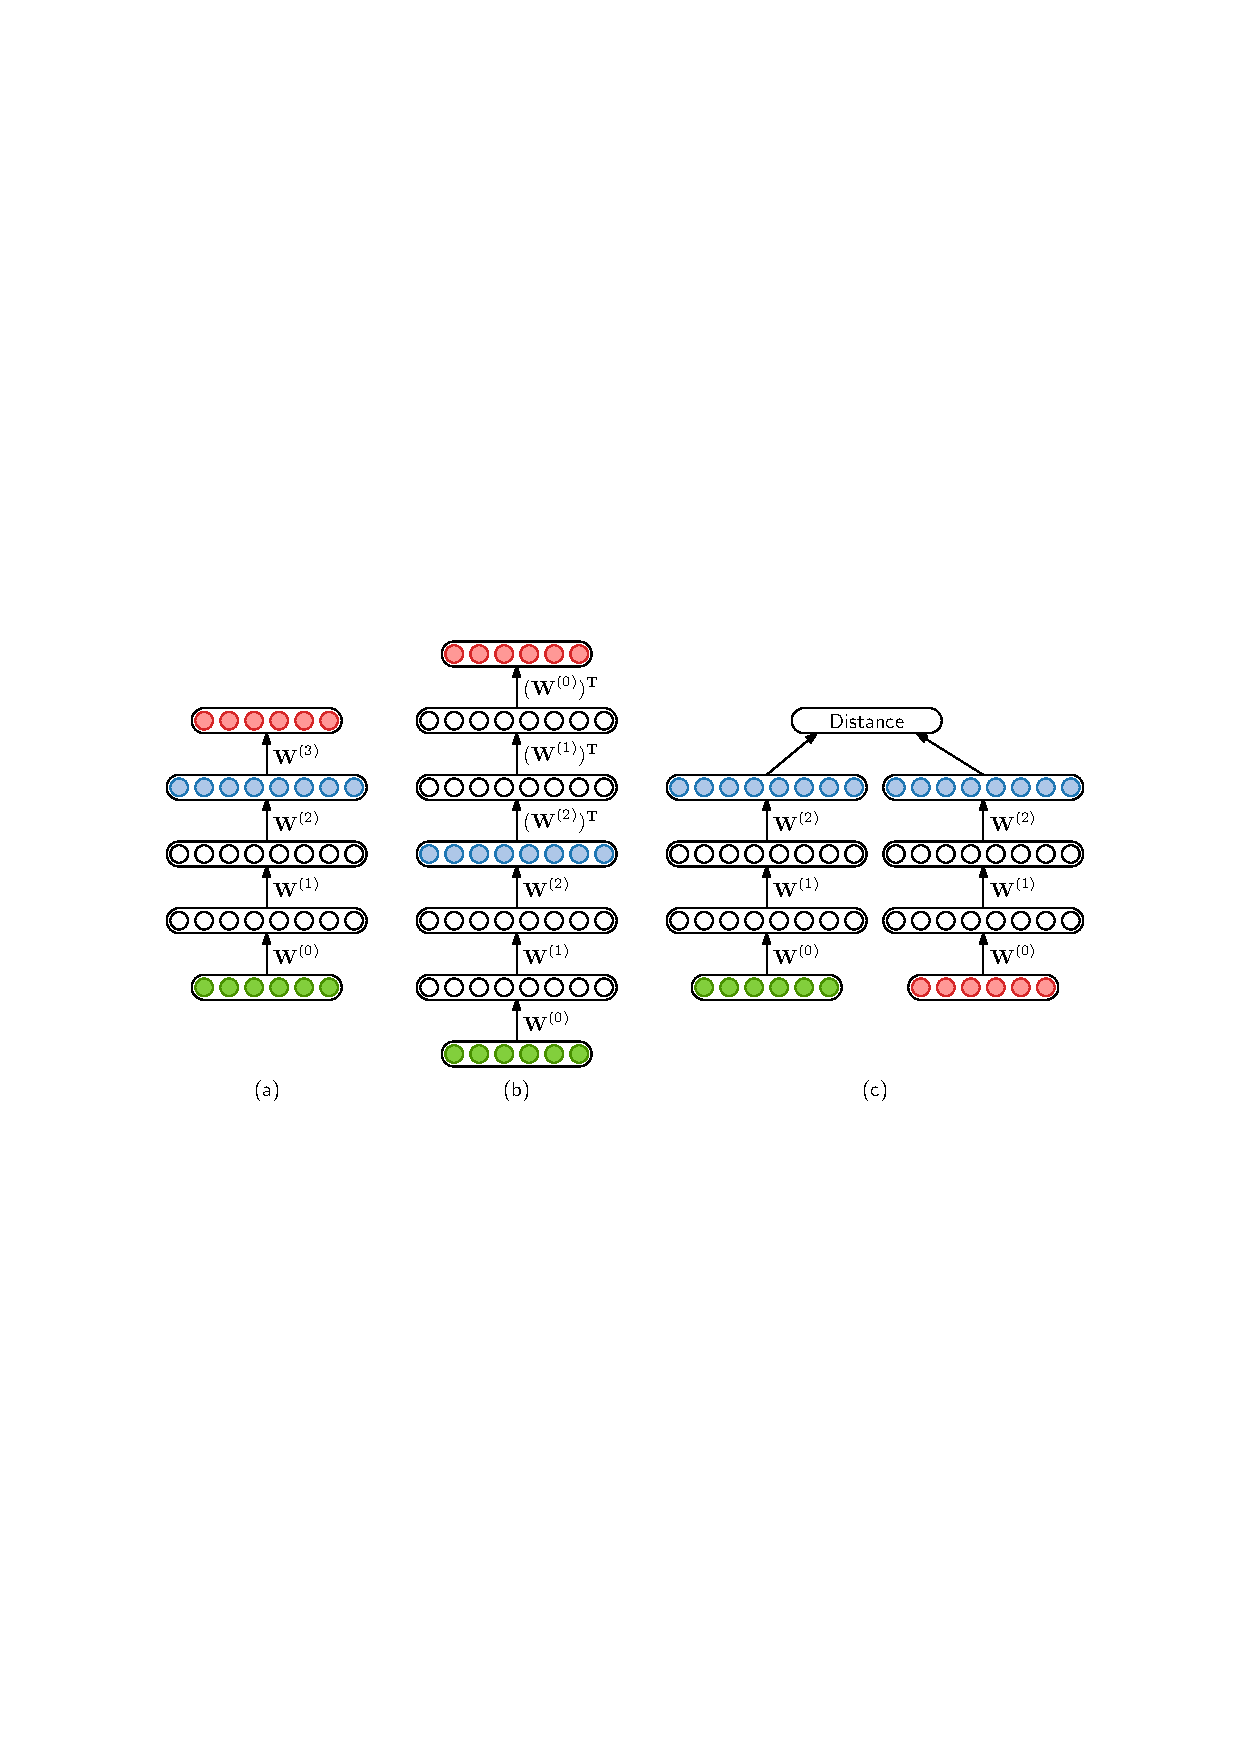
\includegraphics[width=\linewidth]{cae_siamese}
%     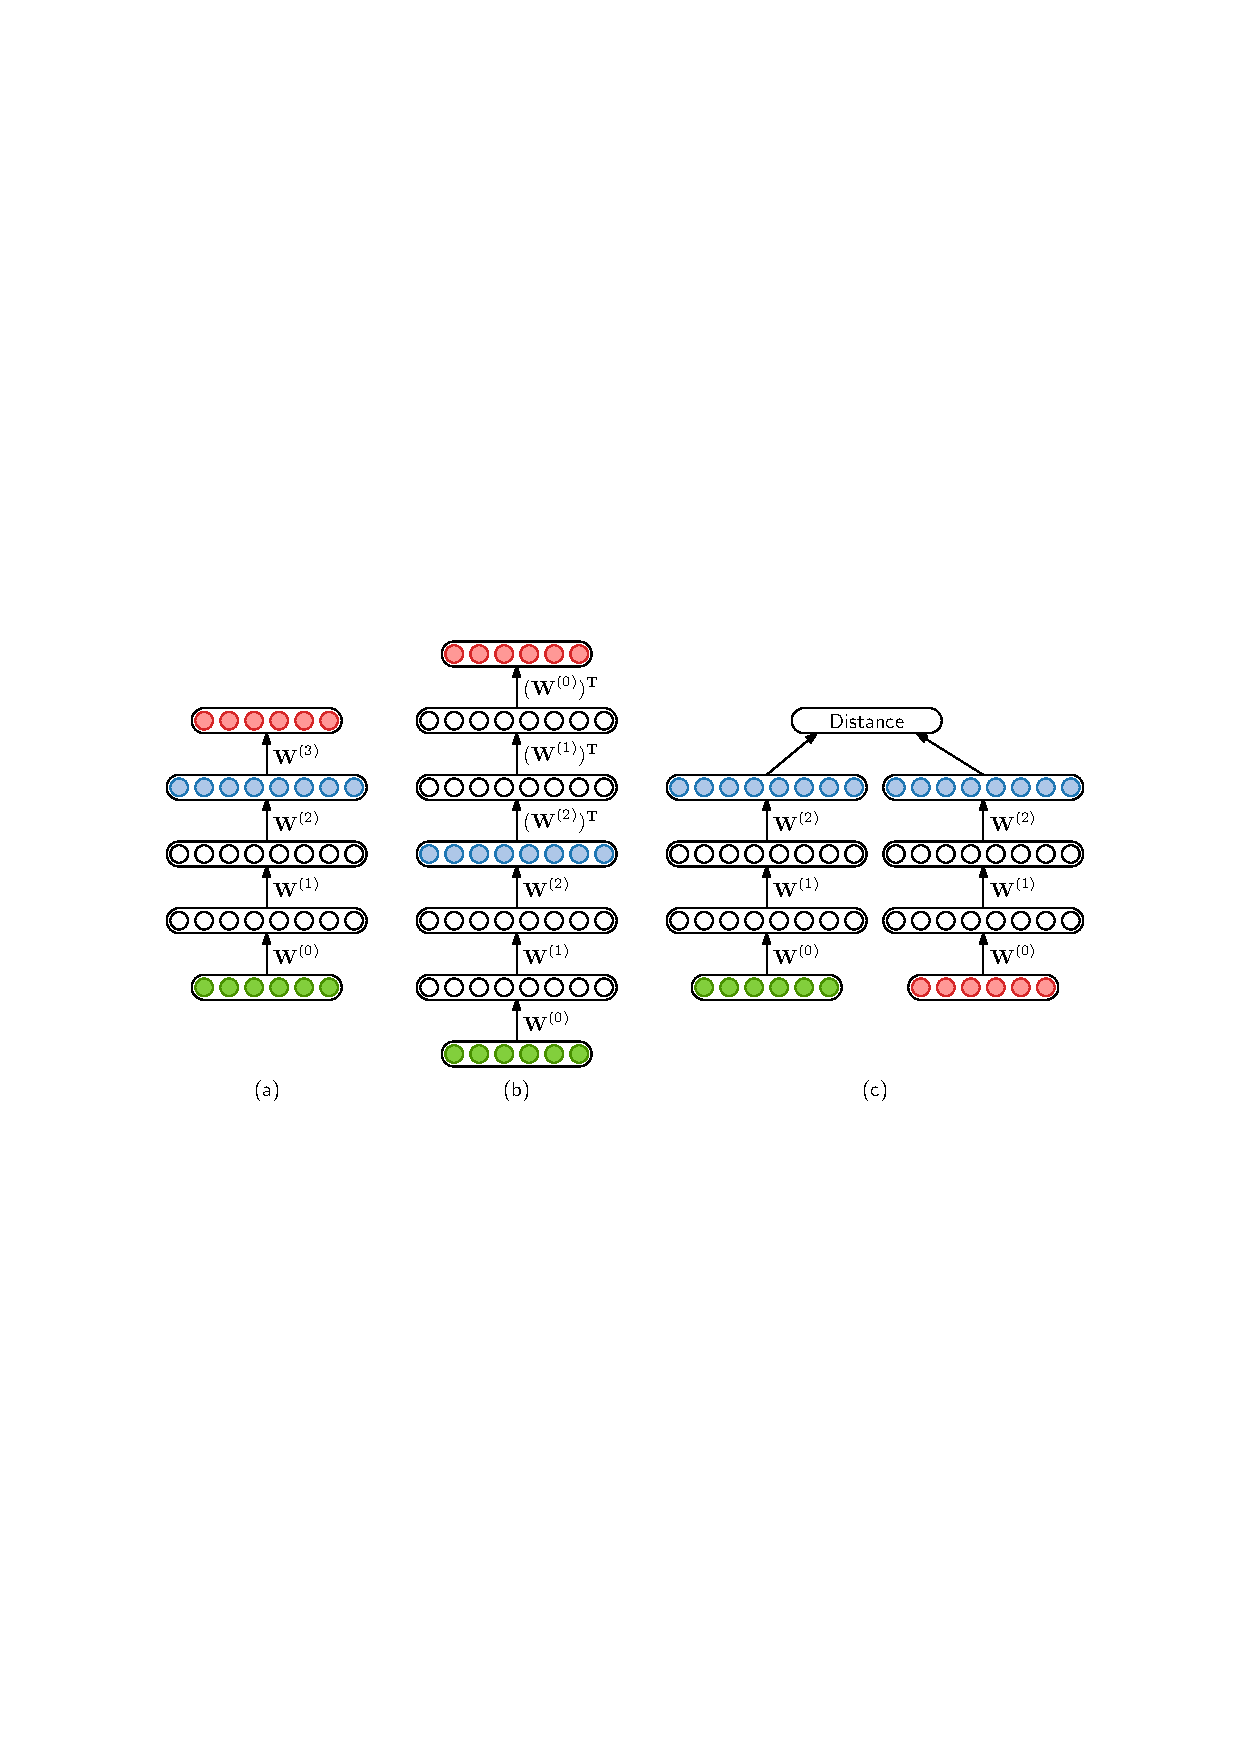
\includegraphics[width=0.918\linewidth]{cae_siamese}
%     \caption[I am the short caption that appears in the list of figures, without references.]{
%     (a) The cAE as used in this chapter. The encoding layer (blue) is chosen based on performance on a development set.
%     (b) The cAE with symmetrical tied weights. The encoding from the middle layer (blue) is always used.
%     (c) The siamese DNN. The cosine distance between aligned frames (green and red) is either minimized or maximized depending on whether the frames belong to the same (discovered) word or not.
%     A cAE can be seen as a type of DNN~\cite{dahl+etal_taslp12}.
%     }
%     \label{fig:cae_siamese}
% \end{figure}


% The following is an example of an equation:
% \begin{equation}
% P(\vec{z} | \vec{\alpha}) = \int_{\vec{\pi}} P(\vec{z} | \vec{\pi}) \, p(\vec{\pi} | \vec{\alpha}) \, \textrm{d} \vec{\pi}
% = \int_{\vec{\pi}} \prod_{k = 1}^K \pi_k^{N_k} \frac{1}{B(\vec{\alpha})} \prod_{k = 1}^K \pi_k^{\alpha_k - 1} \, \textrm{d} \vec{\pi}
% \label{eq:example_equation}
% \end{equation}
% which you can subsequently refer to as~\eqref{eq:example_equation} or Equation~\ref{eq:example_equation}.
% But make sure to consistently use the one or the other (and not mix the two ways of referring to equations).


